\documentclass[a4paper,12pt]{article}

\usepackage[utf8]{inputenc}
\usepackage[T1]{fontenc}
\usepackage[english]{babel}
\usepackage{geometry}
\geometry{a4paper, margin=1in}
\usepackage{amsmath,amssymb}
\usepackage{booktabs,tabularx}
\usepackage{graphicx}
\usepackage{float}
\usepackage{hyperref}
\usepackage{enumitem}
\usepackage{longtable}

\title{Machine Learning Course Project Report\\Text Classification on AG News}
\author{
Tran Hoang Vy Khang (2352502)\\
Le Tan Minh Khoa (2352563)\\
Tao Nguyen Quang Khang (2352499)\\
Tran Gia Huy (2252264)\\
Vo Le Hai Dang (2352257)
}
\date{Semester I, 2025--2026}

\begin{document}

\maketitle

\section{Course Context}
\begin{itemize}[leftmargin=*]
    \item Course: Machine Learning (CO3117)
    \item Department: Computer Science and Engineering, HCMUT -- VNU-HCM
    \item Supervisor: Dr. Le Thanh Sach
    \item Topic: Text Data Classification (Topic 2)
\end{itemize}

\section{Project Objectives}
The project aims to build a complete text classification pipeline from exploratory data analysis to final model comparison, following the required workflow:
\begin{enumerate}[leftmargin=*]
    \item EDA and data understanding.
    \item Configurable preprocessing and TF-IDF feature extraction.
    \item Classical ML training and evaluation (Logistic Regression, SVM, Naive Bayes).
    \item Modern embedding extension with SBERT.
    \item Comparison across feature families with report-ready artifacts.
\end{enumerate}

\section{Dataset and Problem Setting}
\begin{itemize}[leftmargin=*]
    \item Dataset: \texttt{ag\_news} from Hugging Face Datasets.
    \item Task: 4-class news topic classification.
    \item Split used in full mode: 120,000 training samples and 7,600 test samples.
\end{itemize}

\section{Implemented Methodology}
\subsection{Traditional Pipeline}
\begin{itemize}[leftmargin=*]
    \item Preprocessing options: lowercasing, stopword removal, punctuation removal, number removal.
    \item TF-IDF configuration search over three candidates:
    \begin{itemize}
        \item \texttt{tfidf\_uni\_1k}
        \item \texttt{tfidf\_uni\_bi\_3k}
        \item \texttt{tfidf\_uni\_bi\_5k}
    \end{itemize}
    \item Primary model-selection metric: F1-weighted.
    \item Trained models: Logistic Regression, SVM, Naive Bayes.
\end{itemize}

\subsection{Modern Embedding Extension}
\begin{itemize}[leftmargin=*]
    \item Embedding model: \texttt{sentence-transformers/all-MiniLM-L6-v2}.
    \item Benchmark scales: \texttt{5k\_2k} and \texttt{20k\_2k}.
    \item Embeddings and labels are exported to \texttt{.npy} artifacts.
\end{itemize}

\section{Engineering Workflow Integration}
A one-entry workflow was implemented to improve reproducibility:
\begin{itemize}[leftmargin=*]
    \item Planner chooses objective-specific strategy (fast, balanced, best).
    \item Runners execute TF-IDF and embedding branches.
    \item Critic validates quality thresholds, required scales, and artifacts.
    \item Reporter generates concise recommendation outputs.
\end{itemize}

\section{Results}
\subsection{Best TF-IDF Results (Full Data)}
\begin{table}[H]
\centering
\begin{tabular}{lcccc}
\toprule
Model & Accuracy & Precision (w) & Recall (w) & F1 (w) \\
\midrule
SVM & 0.9046 & 0.9044 & 0.9046 & 0.9044 \\
Logistic Regression & 0.9038 & 0.9036 & 0.9038 & 0.9036 \\
Naive Bayes & 0.8871 & 0.8866 & 0.8871 & 0.8867 \\
\bottomrule
\end{tabular}
\caption{TF-IDF model comparison from \texttt{results/tables/tfidf\_model\_comparison.csv}.}
\end{table}

\subsection{SBERT Benchmark Results}
\begin{table}[H]
\centering
\begin{tabular}{lccccc}
\toprule
Scale & Best Model & Accuracy & Precision (w) & Recall (w) & F1 (w) \\
\midrule
5k\_2k & Logistic Regression & 0.8740 & 0.8734 & 0.8740 & 0.8736 \\
20k\_2k & SVM & 0.8955 & 0.8958 & 0.8955 & 0.8954 \\
\bottomrule
\end{tabular}
\caption{Best embedding model per scale from \texttt{results/tables/bert\_benchmark\_summary.csv}.}
\end{table}

\subsection{Feature-Family Comparison}
The final comparison between best TF-IDF and best embedding model shows:
\begin{itemize}[leftmargin=*]
    \item Best TF-IDF: SVM with F1-weighted = 0.9044.
    \item Best embedding: SVM at 20k\_2k with F1 = 0.8954.
\end{itemize}
Therefore, TF-IDF + SVM is selected as the final recommendation for this dataset and setup.

\section{Artifact Outputs}
The project exports reproducible artifacts under \texttt{features/} and \texttt{results/}, including:
\begin{itemize}[leftmargin=*]
    \item Feature arrays (TF-IDF and SBERT) in \texttt{.npy} format.
    \item Confusion matrices for all TF-IDF models.
    \item Benchmark and comparison CSV tables.
    \item Workflow logs, critic report, and reporter summary.
\end{itemize}

\begin{figure}[H]
    \centering
    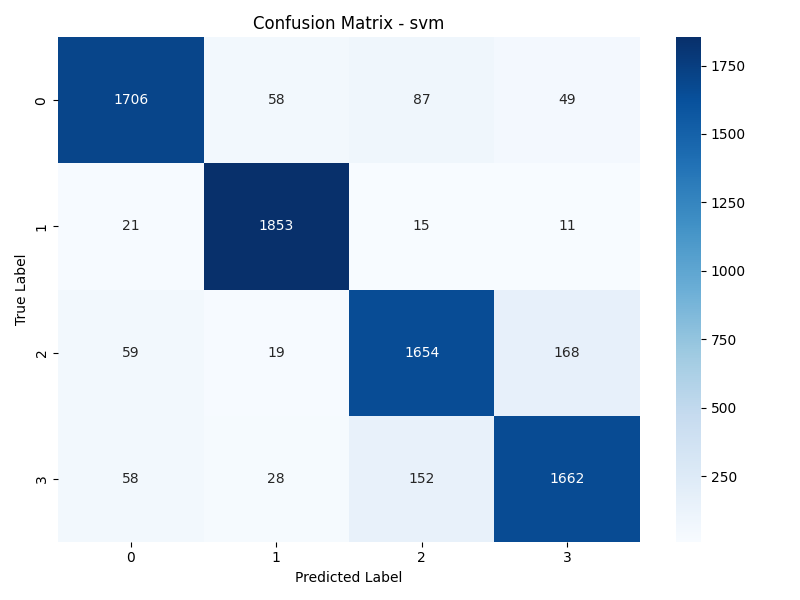
\includegraphics[width=0.65\linewidth]{../results/figures/cm_svm.png}
    \caption{Confusion matrix of best TF-IDF model (SVM).}
\end{figure}

\section{Team Contributions}
\begin{table}[H]
\centering
\begin{tabularx}{\linewidth}{l c X c}
\toprule
Member & ID & Main Contribution & \% \\
\midrule
Tran Hoang Vy Khang & 2352502 & Embedding benchmark, integrated workflow, final comparison and outputs & 30 \\
Le Tan Minh Khoa & 2352563 & Text cleaning and TF-IDF feature engineering & 20 \\
Tao Nguyen Quang Khang & 2352499 & Classical model training and evaluation on TF-IDF & 20 \\
Tran Gia Huy & 2252264 & Pipeline/configuration support and reproducibility structure & 15 \\
Vo Le Hai Dang & 2352257 & Data loading and EDA notebook analysis & 15 \\
\bottomrule
\end{tabularx}
\caption{Detailed contribution table (sum = 100\%).}
\end{table}

\section{Conclusion}
The required course targets were completed:
\begin{itemize}[leftmargin=*]
    \item Complete traditional ML pipeline implemented and validated.
    \item Modern embedding extension benchmarked at multiple scales.
    \item Direct TF-IDF vs embedding comparison produced.
    \item Automated planner-runner-critic-reporter workflow built for reproducibility.
\end{itemize}
Final recommendation: use TF-IDF with SVM as the primary baseline for AG News in this project.

\end{document}
